%!TEX root = ComputerScienceOne.tex

%File IO - exercises

\section{Exercises}

\begin{exer}
Write a function that takes a string representing a file name and
opens and processes the file, returning all of its contents as a single
string.
\end{exer}

\begin{exer}
Consider an irregular, 2-D simple polygon with $n$ points, 
$(x_1, y_1), (x_2, y_2), \ldots, (x_n, y_n)$.  The area $A$ of the 
polygon can be computed as
$$A = \frac{1}{2} \sum_{i=0}^{n-1} (x_iy_{i+1} - x_{i+1}y_i)$$
Note, that the initial and end point will be the same, $(x_0, y_0) =
(x_n,y_n)$.  An example polygon for $n = 5$ can be found in 
Figure \ref{fig:polygonEx}.

\begin{figure}[h]
\centering
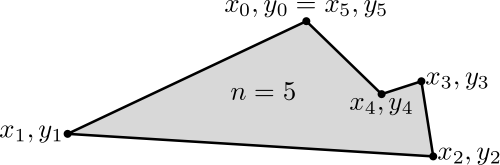
\includegraphics[scale=.5]{images/polygonEx}
\caption{An example polygon for $n=5$}
\label{fig:polygonEx}
\end{figure}

Write a program to open and process a text file containing
$n$ coordinates.  In particular, the first line is a single integer 
$n$ that indicates how many points should be read in.  Each 
line after that has the $x, y$ coordinates of each point separated 
by a single space.

\begin{minted}{text}
4
1.0 0.0
13.2 1.25
20.5 18.4
16.37 24.54
\end{minted}

After reading the file in, it will compute the area of the polygon 
according to the formula above and output it to the user.  For example, 
the output for the above file may be something like \mintinline{text}{Area of the polygon: 197.9135}
\end{exer}

\begin{exer}
Write a program that processes an input text file and scrubs it
of any HTML characters that need to be escaped (see Exercise
\ref{exercise:strings:htmlScrubber} for details).  It should
produce a new output file with all special characters escaped.
\end{exer}

\begin{exer}
Write a program that spell checks a plain text file.  The program
will open a text file and process each word separately, checking 
for proper spelling against a standard dictionary.  

You may assume that each word is separated by some whitespace 
(you may assume that there are no multi-line hyphenated words).  
However, you should ignore all punctuation (periods, question marks, etc.).

Use a standard American dictionary provided on your unix system
which stores words one per line.  Your output should include all
misspelled or unrecognized words (words not contained in the dictionary 
file).
\end{exer}

\begin{exer}
A standard word search consists of an $n \times n$ grid in which there 
are a number of words hidden, some intersecting, with dummy letters 
filling in the blanks.  An example is provided in Figure \ref{fig:wordSearch}.

\begin{figure}[h]
\centering
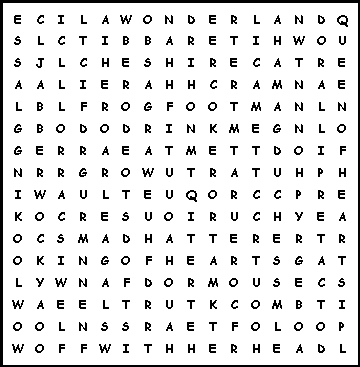
\includegraphics[scale=0.50]{images/wordSearch}
\caption{A Word Search}
\label{fig:wordSearch}
\end{figure}

Write a program to solve a word search.  Your program will read in
an input file with the following format: the first line will contain a 
single integer $n$ which is followed by $n$ lines with $n$ characters 
(not including the end line character) corresponding to the word search.

Once you read in the word search, you will iterate through all possible 
words running down, right, or diagonally down-right.  You will attempt 
to match each possibility against a standard English dictionary.
If the word matches a word in the dictionary, output it to the standard 
output, otherwise ignore it.  To simplify, you may restrict your attention 
to words that have a length between 3 and 8 (inclusive).
\end{exer}

\begin{exer}
Write a crossword puzzle cheater.  The program will take, as input, 
a ``partial'' word in a crossword puzzle.  That is, some of the letters
are known (from other solved clues) while some of the letters are 
not known.  For the purposes of this exercise, we'll use a hyphen 
as a placeholder for missing letters.  

Your program will match the partial word against words in a standard
English dictionary and list all possible matches.  For example, if the 
user provided \mintinline{text}{foo-} as input it might match 
\mintinline{text}{food}, \mintinline{text}{fool}, and \mintinline{text}{foot}.  
\end{exer}

\begin{exer}
Bridge is a four player (2 team) game played with a standard 52-card 
deck.  Prior to play, a round of bidding is performed to determine which 
team is playing for or against the contract, the trump suit, and at what 
level.  Understanding the rules of the game or the bidding conventions 
involved are not necessary for this exercise.  Instead, write a program 
to assist players in how they should bid based on the following point 
system.

A standard 52-card deck is dealt evenly to 4 different hands (Players 
1 thru 4, 13 cards each).  Each player's hand is worth a number of 
points based on the following rules:
\begin{itemize}
  \item Each Ace in the hand is worth 4 points
  \item Each King is worth 3
  \item Each Queen is worth 2
  \item Each Jack is worth 1
  \item For each suit (Diamond, Spade, Club, Heart) such that the hand has only 2 cards (a ``doubleton'') an additional point is added
  \item For each suit that the hand has only 1 card in (a ``singleton'') two additional points are added
  \item For each suit that the hand has no cards (a ``void'') 3 additional points are added.
\end{itemize}
Write a program that reads in a text file containing a deal.  The formatting 
is as follows: the input file will have 4 lines, one for each player.  Each 
line contains the cards dealt to that player delimited by a single space.  
The cards are indicated by the rank ($A, K, Q, J, 10, 9, \ldots, 2$) and 
the suit (D, S, C, H).  An example:

\begin{minted}{text}
3C 3D 7S QD KC AS 6S AC JS 4S JD 7H 6D
5D 8C 7D AH 3H QC 8D JH 5H 9D 7C 9C 4D
2H 10D 8H KS QH 4C 10S 9S 6H 8S KD AD QS
2D 10C 6C 2C 10H 4H 2S 3S 5C 9H KH JC 5S
\end{minted}

Your program should process the file and output the total number 
of points each hand represents.  You should not make any assumptions 
about the ordering of the input.

\begin{minted}{text}
Hand 1 Points: 17
Hand 2 Points: 10
Hand 3 Points: 16
Hand 4 Points: 6
\end{minted}
\end{exer}

\begin{exer}
The game of Sudoku is played on a $9 \times 9$ grid in which
entries consist of the numbers 1 thru 9.  Initially, the board is 
presented with some values filled in and others blank.  The player 
has to fill in the remaining values until all grid boxes are filled and
the following constraints are satisfied.
\begin{itemize}
  \item In each of the 9 rows, each number, 1--9 must appear exactly once
  \item In each of the 9 columns, each number 1--9 must appear exactly once
  \item In each of the $3 \times 3$ sub-grids, each number 1--9 must appear exactly once
\end{itemize}
A full example is presented in Figure \ref{fig:sudoku01}.
\begin{figure}[h]
\centering
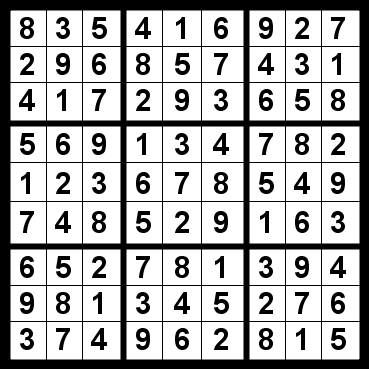
\includegraphics[scale=0.50]{images/sudoku01.png}
\caption{A solved Sudoku puzzle}
\label{fig:sudoku01}
\end{figure}

Write a program that processes a text file containing a possible 
sudoku solution and determine if it is a \emph{valid} or \emph{invalid} 
solution.  The file will have the following format: it will contain 9 lines 
with 9 numbers on each line delimited by a single space.  If the input 
represents a valid solution, output "Valid Solution", otherwise output at 
least one reason why the input is not a valid solution.
\end{exer}

\begin{exer}
Write a program that parses and processes a data file containing 
Comma Separated Values (CSV) and produce an equivalent
JSON (JavaScript Object Notation) output file containing the same 
data.  

The input file will have the following format.  The first line is a CSV 
list of column names.  Each subsequent line is an individual record 
with values for each column. The number of columns and rows may 
vary from file to file.  The following is an example containing data 
about students, which has four columns and 3 records.

\begin{minted}{text}
lastName,firstName,NUID,GPA
Castro,Starlin,11223344,3.48
Rizzo,Anthony,55667788,3.95
Bryant,Chris,01234567,2.7
\end{minted}

The output file will be formatted in JSON where each ``object'' 
(record) is denoted with opening and closing curly brackets, each 
record is separated by a comma, and all records are enclosed in 
square brackets (putting them in an array).  For each record, each 
value is denoted with a key (the column name) and a value.  For
this exercise, treat all values as strings even if they are numbers.  
For example, the input file above would be formatted as follows.

\begin{minted}{json}
[
  {
    "lastName": "Castro",
    "firstName": "Starlin",
    "NUID": "11223344",
    "GPA": "3.48"
  },
  {
    "lastName": "Rizzo",
    "firstName": "Anthony",
    "NUID": "55667788",
    "GPA": "3.95"
  },
  {
    "lastName": "Bryant",
    "firstName": "Chris",
    "NUID": "01234567",
    "GPA": "2.7"
  }
]
\end{minted}

\end{exer}

\begin{exer}

TODO: move this to sorting?

Data has a ``natural'' ordering: numbers are ordered in nondecreasing 
order, strings are ordered lexicographically (according to the ASCII text 
table).  However, in many situations, the natural ordering isn't the 
\emph{expected} ordering.  For example, class years are usually ordered Freshman, Sophomore, Junior, Senior whereas the natural ordering 
would order them Freshman, Junior, Senior, Sophomore.  

Write a program to sort a collection of strings according to 
an arbitrary artificial ordering.  That is, instead of the A--Z 
alphabetic ordering, we will order them according to an alternative 
ordering of the English alphabet.  As an example, one possible
ordering would be:

\mintinline{text}{n e d c r h a l g k m z f w j o b v x q y i p u s t}

Your job will be to \emph{sort} a list of English language words 
using this artificial ordering of the English alphabet.  Specifically, 
you will read in an input file in the following format.  The first line 
is the new ordering of English letters, each separated by a space.  
Each line after that contains a single string.  
You will read in this file, process it and produce a reordered list 
of the words sorted according to the new ordering.  

An example input:

\begin{minted}{text}
n e d c r h a l g k m z f w j o b v x q y i p u s t
vcawufotrb
laencfuesw
gvtkwekfom
vrsfqictqc
wmcvmjmtet
qetegyqelu
newaxdtjlt
nfrfrwkknj
fzqrvgblov
gkkmgwwwpa
\end{minted}

The result ordering: 

\begin{minted}{text}
Artificial Ordering: 
newaxdtjlt
nfrfrwkknj
laencfuesw
gkkmgwwwpa
gvtkwekfom
fzqrvgblov
wmcvmjmtet
vcawufotrb
vrsfqictqc
qetegyqelu
\end{minted}

For simplicity, you can assume that all words will be lower 
case and no non-alphabetic characters are used.  However, 
you may not assume that all words will be the same length. 
Words of a shorter length that are a prefix of another word 
should be ordered first.  For example, ``newax'' should come 
before ``newaxn'' in the ordering above.
\end{exer}

\begin{exer}
Ranked voting elections are elections where each voter 
\emph{ranks} each candidate rather than just voting for a 
single candidate.  If there are $n$ candidates, then each
voter will rank them 1 (best) through $n$ (worst).  Usually, 
the winner of such an election is determined by a 
\emph{Condorcet} method (the candidate that would
win in by a majority in all head-to-head contests).  
However, we'll use an alternative method, a \emph{Borda count}.

In a Borda count, points are awarded to each candidate 
for each ballot.  For every number 1 ranking, a candidate 
receives $n$ points, for every 2 ranking, a candidate gets 
$n-1$ points, and so on.  For a rank of $n$, the candidate 
only receives 1 point.  The candidates are then ordered by 
their total points and the one with the highest point count 
wins the election.  Such a system usually leads to a 
``consensus'' candidate rather than one preferred by a 
majority.

Implement a Borda-count based ranked voting program.  
Your program will read in a file in the following format.  
The first line will contain an ordered list of candidates 
delimited by commas.  Each line after that will represent 
a single ballot's ranking of the candidates and will contain 
comma delimited integers 1 through $n$.  The order of 
the rankings will correspond to the order of the candidates 
on the first line.

Your program will take an input file name as a command 
line argument, open the file and process it.  It will then 
report the results including the point total for each candidate 
(in order) as well as the overall winner.  It will also report the
total number of ballots.  You may assume each ballot is 
valid and all rankings are provided.

An example input:

\begin{minted}{text}
Alice,Bob,Charlie,Deb
2,1,4,3
3,4,2,1
4,2,3,1
3,2,1,4
3,1,4,2
\end{minted}

An example output:

\begin{minted}{text}
Election Results
Number of ballots: 5

Candidate  Points
Bob        15
Deb   	   14
Charlie    11
Alice      10

Winner is Bob
\end{minted}
\end{exer}

\begin{exer} 
A DNA sequence is a sequence of some combination of the 
characters \mintinline{text}{A} (adenine), \mintinline{text}{C} (cytosine), 
\mintinline{text}{G} (guanine), and \mintinline{text}{T} (thymine) 
which correspond to the four nucleobases that make up DNA.  
Given a long DNA sequence, its often useful to compute the 
frequency of \emph{n-grams}.  An $n$-gram is a DNA subsequence 
of length $n$.  Since there are four bases, there are $4^n$ possible 
$n$-grams.

Write a program that processes a DNA sequence from a plaintext
file and, given $n$, computes the relative frequency of each $n$-gram 
as it appears in the sequence.  As an example, consider the sequence in Figure \ref{figure:dnaSequence}.

\begin{figure}[h]
\centering
\mintinline{text}{GGAAGTAGCAGGCCGCATGCTTGGAGGTAAAGTTCATGGTTCCCTGGCCC}
\caption{A DNA Sequence}
\label{figure:dnaSequence}
\end{figure}

To compute the frequency of all $n=2$ $n$-grams, we would 
consider all 16 combinations of length-two DNA sequences.  We 
would then go through the sequence and count up the number of 
times each $2$-gram appears.  We then compute the relative 
frequency (note: if a sequence is length $L$, then the total number 
of $n$-grams in it is $L - (n - 1)$).  The relative frequency of each 
such $2$-gram is calculated below.

\begin{minted}{text}
AA  6.1224%
AC  0.0000%
AG 10.2041%
AT  4.0816%
CA  6.1224%
CC 10.2041%
CG  2.0408%
CT  4.0816%
GA  4.0816%
GC 10.2041%
GG 12.2449%
GT  8.1633%
TA  4.0816%
TC  4.0816%
TG  8.1633%
TT  6.1224%
\end{minted}
\end{exer}

\begin{exer}
Given a long DNA sequence, it is often useful to compute
the number of instances of a certain \emph{subsequence}.
As an example, if we were to search for the subsequence 
$GTA$ in the DNA sequence in Figure \ref{figure:dnaSequence}, 
it appears twice.  As another example, in the sequence 
\mintinline{text}{CCCC}, the subsequence \mintinline{text}{CC} 
appears three times.

Write a program that processes a text file containing a DNA
sequence and, given a subequence $s$, searches the DNA 
sequence and counts the number of times $s$ appears.
\end{exer}

\begin{exer}
Protein sequencing in an organism consists of a two step 
process.  First the DNA is translated into RNA by replacing 
each thymine (T) nucleotide with uracil (U).  Then, the RNA 
sequence is translated into a protein according to the following 
rules.  The RNA sequence is processed 3 bases at a time.  
Each \emph{trigram} is translated into a single amino acid
according to known encoding rules.  There are 20 such amino 
acids, each represented by a single letter in $(A,C,D,E,F,G,H,I,K,L,M,N,P,Q,R,S,T,V,W,Y)$.

The rules for translating trigrams are presented in Figure 
\ref{figure:codonTable}.  Each triple defines a protein, 
but we're only interested in the first letter of each protein.
Moreover, the trigrams UAA, UAG, and UGA are special 
markers that indicate a (premature) end to the protein 
sequencing (there may be additional nucleotides left in the 
RNA sequence, but they are ignored and the translation 
ends).  

\begin{figure}[h]
\centering
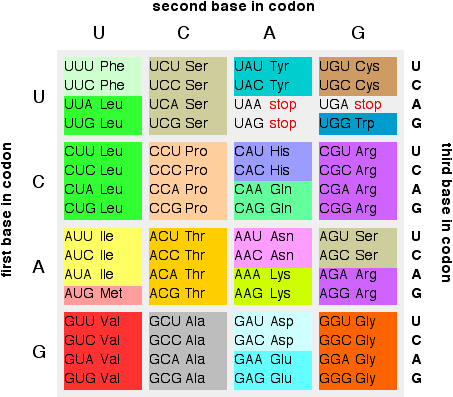
\includegraphics[scale=0.65]{images/codonTable}
\caption{Codon Table for RNA to Protein Translation}
\label{figure:codonTable}
\end{figure}

As an example, suppose we start with the DNA sequence 
$AAATTCCGCGTACCC$; it would be encoded into RNA
as $AAAUUCCGCGUACCC$; and into an amino acid 
sequence $KFRVP$.

Write a program that processes a file containing a DNA
sequence and outputs the translated proteins (only the
first letter of each protein) to an output file.
\end{exer}

\begin{exer}
Recently, researchers have successfully inserted two new 
artificial nucleases into simple bacteria that successfully 
reproduced the artificial bases through several generations.  
The artificial bases d5SICS and dNaM, ($X$ and
$Y$ for short) mimic the natural $G$, and $C$ nucleobases 
respectively.  

Write a program that takes a normal DNA sequence and replace 
some of its $G, C$ pairs with $X, Y$ respectively.  DNA is translated 
into RNA which is then translated into 20 different amino acids.  
Each amino acid produced depends on a 3 nucleobase \emph{codon}.  
For this exercise, we will change $G, C$ pairs with $X, Y$ pairs but
only in codons that represent the amino acids Threonine (an 
essential amino acid) and Alanine (a non-essential amino acid).
Table \ref{table:aminoAcids} contains the codons corresponding 
to these amino acids and the codons you  should translate each one 
to.  All other codons should not be modified.

Your program should open and process a DNA sequence contained in
a file and modify the DNA sequence as described above and output
the artificial DNA sequence to a new output file.  

\begin{table}[h]
\center
\begin{tabular}{|c|c|c|}
\hline
Amino Acid & Codon & Artificial Codon \\
\hline
\hline
\multirow{4}{*}{Threonine} & ACT & AYT \\
~& ACC & AYY \\
~& ACA & AYA \\
~& ACG & AYX\\
\hline
\multirow{4}{*}{Alanine} & GCT & XYT \\
~& GCC & XYY \\
~& GCA & XYA \\
~& GCG & XYX \\
\hline
\end{tabular}
\caption{Amino Acid Codons}
\label{table:aminoAcids}
\end{table}
\end{exer}


